\chapter{Robotic Volatile Sampling for Early Detection of Plant Stress}
\label{ch:VOL}


\author{Christian Geckeler$^{1,2,*}$, Sergio E. Ramos$^{3, *}$, Meredith C. Schuman$^{3}$, and Stefano Mintchev$^{1,2}$
        % <-this % stops a space
%\thanks{This work was supported by the Syngenta-PSC Fellowships and the SNSF Eccellenza Grant N.186865.}% <-this % stops a space
\thanks{${}^{1}$Environmental Robotics Laboratory,
ETH Zurich, Switzerland.}%
\thanks{${}^{2}$Swiss Federal Institute for Forest, Snow, and Landscape Research.}
\thanks{${}^{3}$Spatial Genetics, University of Zurich, Switzerland.}%
\thanks{${}^{*}$Denotes equal contribution}
\thanks{Supplementary material available at: \href{https://doi.org/10.3929/ethz-b-000619903}{10.3929/ethz-b-000619903}}
}

\begin{abstract}
Global agriculture is challenged to provide food for a human population that is larger than ever before, and still increasing. This is accompanied by the need to reduce the large global impacts of agriculture while increasing yields. Early identification of plant stress enables fast intervention to limit crop losses, and optimized application of pesticides and fertilizer to reduce environmental impacts. Current image-based approaches identify plant stress responses hours or days after the stress event, usually only after substantial damage has occurred and visual cues become apparent. In contrast, plant volatiles are released seconds to hours after stress events, and can quickly indicate both the type and severity of stress. An automatable and non-disruptive sampling method is needed to enable the use of plant volatiles for monitoring plant stress in precision agriculture. In this work, we detail the development of a plant volatile sampler that can be deployed and collected with an uncrewed aerial vehicle. The effect of sampling flow rate, horizontal distance to volatile source, and overhead downwash on collected volatiles is investigated, along with the deployment accuracy and retrieval successes with manual flight. Finally, volatile sampling is validated in outdoor tests. The possibility of robotic collection of plant volatiles is a first and important step towards the use of chemical signals for early stress detection and opens up new avenues for precision agriculture beyond visual remote sensing.
\end{abstract}

% \begin{IEEEkeywords}
% Plant volatiles, Precision agriculture, Robotic sampling, Aerial Robots, Sensor delivery, Sensor Retrieval, Remote sensing
% \end{IEEEkeywords}

\section{Introduction}

Global agriculture faces unprecedented pressures to feed a growing population, cater to increasingly selective consumer choices, ensure economic viability for the roughly one billion farmers in the world, ensure enough yield with increasingly unpredictable and extreme climate events, and also reduce environmental impact~\cite{McGreevy2022}. Through sustainable intensification (SI), large global change impacts of agriculture can be reduced while increasing yields~\cite{Cassman2020, Pretty2018, Garnett2013}. Many SI strategies leverage productivity gains from increasing biodiversity in farm fields, which can improve land area use and conserve soil through better space-filling. However, the cultivation of such heterogeneous SI fields is more labor-intensive per area than for homogeneous monoculture-based approaches, and not amenable to standard automation strategies for monocultures, which require bare soil and synchronized yields. Smart and adaptive automation is thus critical to upscale SI and provide more food on less land, with fewer negative impacts~\cite{Sparrow2021, Basso2020}.

\begin{wrapfigure}{r}{0.5\linewidth}
% \begin{figure}[!t]
\centering
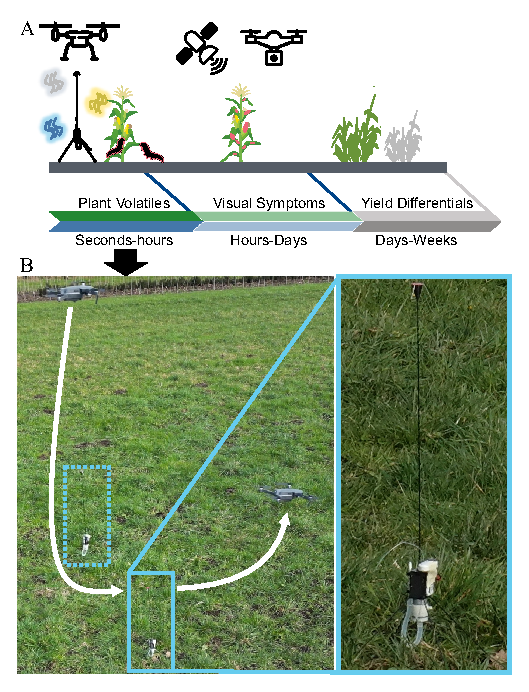
\includegraphics[width=1\columnwidth]{chapters/papers/VOL/figures/fig-1-overview/fig-1-overview.eps}
\caption{Overview of the proposed strategy. (A) Plant stress can be detected orders of magnitude faster (and diagnosed more precisely) using plant volatiles compared to conventional image-based techniques. (B) Deployment with an uncrewed aerial vehicle of the sampler pump for plant volatiles. A video of the deployment and retrieval processes is available as supplementary material.}
\label{fig-1-overview}
% \end{figure}
\end{wrapfigure}

A key challenge for SI is the early detection of plant stress for rapid and effective interventions to reduce crop losses, and to optimize the application of pesticides and fertilizers, thereby reducing environmental impact. Precision agriculture thus far has mainly relied on visual imaging technologies such as multi- or hyperspectral cameras to detect plant stress~\cite{Tsouros2019, Toth2016, Singh2020}. A current limitation is that imaging is best suited to identify plant responses to stress at a later stage, i.e., when plants have already undergone substantial damage, because visual damage appears hours or even days after the stress event~(Figure~\ref{fig-1-overview}A)~\cite{mahlein_hyperspectral_2018}. However, plants respond to stress within seconds to hours by producing phytohormones and bioactive chemicals from a variety of pathways~\cite{schuman_layers_2016}. Some of these have sufficiently low vapor pressure to be volatile under standard conditions on Earth, and thus can be perceived at a distance. One of the best-studied phenomena in the field of plant-insect interactions is the production of specific plant volatile blends upon herbivory (10's to 100's of compounds) which indicate the timing and nature of the herbivore as well as the severity of attack~\cite{howe_plant_2008, dicke_evolutionary_2010}. Plant volatiles thus serve as important indicators of plant condition prior to visible or severe damage, and also can indicate the success or failure of some SI strategies. Plant volatiles have been used by insects and other organisms over millions of years to forage on plants and assess plant status, but they are still not exploited for precision agriculture~\cite{turlings_tritrophic_2018}. Volatiles represent an interesting alternative or complement to imaging for early and precise detection of stress and subsequent application of mitigation strategies to reduce yield loss.

Although there are many established approaches for sampling plant volatiles in the laboratory, it is not trivial to conduct sampling in realistic environments~\cite{lang_ecological_2022,tholl_trends_2021}. As signaling molecules, volatiles are present in relatively low amounts, and they diffuse and can react to form other molecules both in the atmosphere and especially on collection surfaces \cite{dettmer_ambient_2003}. To effectively apply volatile sampling as a method of early plant stress detection, it needs to be repeatable, to minimize mechanical disturbances to the crop, and to scale to cover the spatial and temporal dimensions needed in agriculture. This is not feasible with manual sampling. Mobile robots, in particular Uncrewed Aerial Vehicles (UAVs), present one possible solution. The use of UAVs in agriculture for precision farming is well established, with many commercial systems and services available~\cite{Manfreda2018, Zhang2022}. The company Scentroid offers a UAV-based platform for volatile detection, but it is heavy, requiring large UAVs (DJI Spreading Wings S1000) which generate strong downwash, and available sensors are for inorganic pollutants, methane, particulates, or total Volatile Organic Compounds (VOCs) with no chemical resolution. A UAV system for plant volatile sampling over forest canopies has been described and used for atmospheric monitoring, which is implemented on a large UAV (DJI Matrice 600) causing strong downwash and canopy disturbance (co-opted to mix the sampled air), with sampling exclusively onboard the UAV; this system is also not suited to scalable spatial sampling in precision agriculture \cite{mckinney_sampler_2019}.
%TODO Add more citations, include description of of why deployable sampler

Here we present the initial validation of a method to collect plant volatiles in open air based on samplers deployable from commercial off-the-shelf unmanned aerial vehicles (UAVs)~(Figure~\ref{fig-1-overview}B).
We report the development and characterization of a lightweight plant volatile sampler capable of UAV deployment and collection, with analysis of the effect of sampling flow rate, horizontal (ground) distance between sampler and volatile emission, and overhead downwash (vertical distance). Next, the deployment and retrieval of the sampler with a teleoperated UAV is evaluated, and finally, field tests are conducted which demonstrate the capability of the system to sample volatiles in the open from real maize plants under simulated herbivory.

\section{Collection of Plant Volatiles}

Volatile sampling is achieved by exposing volatiles either to a sorbent, which captures compounds for later analysis, or to a sensor which produces a signal in response to the individual compounds or compound composition~\cite{tholl_trends_2021}. The most sensitive approach is to collect compounds quantitatively by filtering a known volume of air. Once captured on the sorbent, samples can be stored and transported to a laboratory for separation and analysis of individual compounds by gas chromatography and mass spectrometry (GC-MS). Field-portable GC-MS instruments are available, but resolution and sensitivity are generally inversely proportional to size, and no field-portable instruments are comparable in resolving power to laboratory instruments~\cite{tholl_trends_2021, lang_ecological_2022}. Other options for near-real time sensing such as electronic noses or polymer- or metal-based sensors are appropriate once target volatile profiles are known because they provide little or no information about blend composition. These generally also have lower sensitivity than MS and can be more sensitive to environmental fluctuations than simple sample capture \cite{tholl_trends_2021, lang_ecological_2022}. For these reasons, in this study we decided to use a sorbent to collect plant volatiles, and the next sections analyze its integration with a UAV-deployed sampler for remote sampling.

\section{UAV-assisted Collection of Plant Volatiles}

Scalable, sensitive, and non-disruptive sampling of plant volatiles would benefit from customized robotic platforms. While ground robots have the benefit of long sampling times, driving through fields necessitates simple and standardized layouts which may not be present in SI fields, and can also damage plants and alter the released volatile blend. Aerial robots present a more mobile and rapidly deployable solution, capable of quickly reaching remote points in the field while limiting disturbance to plants, especially for small platforms, where the downwash disturbance is small relative to ambient wind. Aerial platforms have the added benefit of easier scaling with plant size, from cover crops to agro-forestry.

There are fundamentally two methods of sampling with a UAV: either attaching the pump directly as previously described~\cite{mckinney_sampler_2019}, or placing and re-collecting a sampler. Attaching the sampling pump directly to the UAV and hovering during sampling presents the simplest solution, but also limits sampling times due to the UAV battery, with potential disturbances to sampling from UAV downwash~\cite{mckinney_sampler_2019}. Landing the UAV with the pump would permit longer sampling times, but entails challenges similar to those for ground robots, as well as crop foliage entering the propellers, and difficulty in landing due to uneven terrain. In addition, this method requires one UAV per sampler, increasing cost and limiting scalability.
By contrast, a deployable sampler can be placed, sample over a desired period of time, and then be re-collected. This minimizes plant disturbance, allows the sampler to sample for any desired period with pre-programmed timing (e.g., starting with a delay after deployment to limit disturbance effects from the UAV), and also permits one UAV to deploy multiple samplers. The following sections details the design of the sampler, and the deployment and retrieval mechanisms (Figure~\ref{fig-3-pump-collection}). Since the current focus is on the sampler mechanism, the UAV is teleoperated. However, such an aerial system could be automated, which is the subject of ongoing work.

\begin{figure*}[h!t]
\centering
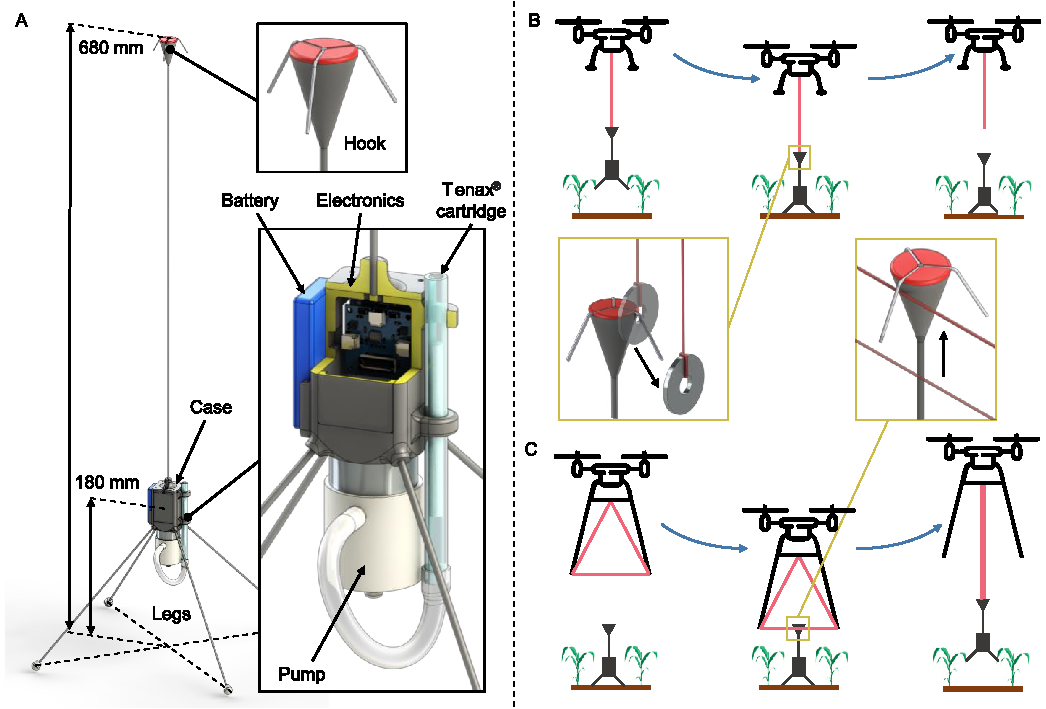
\includegraphics[width=1\columnwidth]{chapters/papers/VOL/figures/fig-3-sampler-pump/fig-3-sampler-pump-v02.eps}
\caption{Sampler design, retrieval and collection methods. (A) The sampler consists of a central case with a battery, control and communication electronics, and a pump connected to a Tenax-TA\textsuperscript{TM} cartridge to sample volatiles. Four legs stabilize the sampler on the ground. Hooks extending above the sampler allow for deployment and retrieval. (B) Deployment occurs when the sampler is lowered by the UAV, which releases the hook from the tether. (C) To retrieve the sampler, the UAV engages a taut wire against the hooks of the sampler, which releases the magnetically-held stretch of the wire and leaves the sampler suspended beneath the UAV. }
\label{fig-3-pump-collection}
\end{figure*}

\subsection{Volatile Sampler Design}
Since the sampler will be deployed by the UAV into the field, it must be self-sufficient during the sampling interval. The sampler consists of a central case, with a pump (Adafruit 4.5V vacuum pump), a battery (SWAYTRONIC LiPo 1S 3.7V 260mAh), control and communication electronics (a Tinyzero processor board, a Dual Motor Tinyshield and a 433MHz Long Range Radio Tinyshield). The pump draws air through a cartridge, which is a glass tube filled with Tenax-TA\textsuperscript{TM}, a porous polymer used as an adsorbent material that traps volatile organic compounds from air or liquids through weak intermolecular binding forces (Figure~\ref{fig-3-pump-collection}A). The pump can be remotely activated via a 433 MHz communication system suitable for medium-sized fields (1 hectare). The user can also remotely set the sampling time and flow rate via the control electronics. Four legs stabilize the sampler, and hooks extending above the sampler provide an attachment point for the UAV during deployment and retrieval. The collection of plant volatiles is commonly done in the early growth phase, when the crop is most sensitive to stress and the canopy is still relatively low~\cite{turlings_tritrophic_2018}. For this reason, we considered it sufficient to position the hooks 680 mm above the ground to retrieve the sampler with the UAV.

The entire sampler weighs 85.9~g, making it suitable for aerial deployment even with small UAVs (weight $<$ 1~kg). Most of the weight is taken by the pump, followed by the electronics and enclosure. For a more detailed weight breakdown of the components, see Figure~\ref{sampler-weight-breakdown}.

\subsection{Delivery and Retrieval System}
There are examples of sensor delivery in tree canopies with UAVs, including the firing of sensor darts \cite{Farinha2020} and the placement of adhesive and coiling sensors with aerial robots \cite{Hamaza2019, Geckeler2022a}, but the delivery and retrieval of sensors in agricultural fields are less explored.

The delivery procedure we propose can be seen in Figure~\ref{fig-3-pump-collection}B. The distinctive feature of this solution is that it requires only passive mechanical systems which can be conveniently integrated into commercially available UAVs. The sampler is hooked to a weighted metal disk at the end of a length of wire attached to the UAV. The length of wire increases the period of oscillation of the sampler and thus reduces the destabilizing effect of the additional weight on the UAV. To deploy the sampler, the UAV descends until the sampler rests on the ground, with the weight of the metal disk disengaging it from the sampler hook (Figure~\ref{fig-3-pump-collection}B, center).


The separate retrieval mechanism consists of a triangle of wire stretched within an inverted Y-shaped frame (Figure~\ref{fig-3-pump-collection}C). The wire is magnetically attached to the ends of the inverted Y-frame. To collect the sampler, the UAV descends until the string is below the hooks, then moves forward until the string engages with the sampler hooks (Figure~\ref{fig-3-pump-collection}C, center). At this point the UAV ascends, with the weight of the sampler disengaging the magnets which hold the string taut, leaving the sampler suspended below the UAV in a similarly stable configuration to the deployment. The red top of the hook assembly allows for easier detection in the camera view for the pilot when aligning for deployment or retrieval. Currently, the retrieval and collection mechanisms must be manually switched. Since retrieval does not immediately follow deployment, this downtime can facilitate the substitution. The passive mechanisms permit fast attachment to off-the-shelf commercial drones, without requiring any additional electrical integration or other customization. For further practical details regarding the deployment procedures, see Section~\ref{robotic_deployment_and_retrieval}.

\begin{figure}[h!t]
\centering
% \documentclass[border=0.2cm]{standalone}
% \documentclass[tikz, convert={density=300,outext=.png}]{standalone} => probably not needed
 
% % Pie chart drawing library 
% \usepackage{pgf-pie}  
 
% \begin{document}

\definecolor{m-blue}    {HTML}{4477AA}
\definecolor{m-cyan}    {HTML}{66CCEE}
\definecolor{m-green}   {HTML}{228833}
\definecolor{m-yellow}  {HTML}{CCBB44}
\definecolor{m-red}     {HTML}{EE6677}
\definecolor{m-purple}  {HTML}{AA3377}
\definecolor{m-grey}    {HTML}{BBBBBB}
 
\begin{tikzpicture} [align=center]
 % \color[HTML]{4477AA}, \color[HTML]{FF7F00}, \color[HTML]{FF7F00}, \color[HTML]{FF7F00}, \color[HTML]{FF7F00}
\pie[scale=0.75, explode=0.1, color={m-blue, m-cyan, m-green, m-yellow, m-red}]{
    42.3/Pump,
    22.3/Electronics and\\ enclosure,
    13.3/Legs and\\ hook assembly,
    11.8/Tenax tube and\\ tubing,
    10.2/Battery} 
\end{tikzpicture}
 
% \end{document}
\caption{Weight breakdown of the sampler: most of the weight is taken by the pump, followed by the electronics. The total weight of the sampler is 85.9~g.}
\label{sampler-weight-breakdown}
\end{figure}

\section{Experimental Results}

\subsection{Sampler Performance Under Different Flow Rates}
%
To evaluate the performance of the sampler in collecting volatile compounds, we compared it to a Gilian GilAir plus (Sensidyne, FL, USA), a  portable pump weighing 580~g that features constant flow and pressure control modes, automatic calibration, and a flow rate of 1 to 5000~ml/min depending on resistance. The GilAir plus and the sampler were compared at the flow rates of 150~ml/min and 200~ml/min. Furthermore, we compared the performance of the sampler under the flow rates of 300 ml/min, 400 ml/min, and 500~ml/min. In all cases, five replicates per flow rate and pump were taken. In both pumps, the flow rate was adjusted with a sorbent tube filled with Tenax-TA\textsuperscript{TM} polymer (Markes Ltd.) attached to account for the pressure needed. We used an external airflow sensor for the flow rate calibrations (Omron Electronic D6F-01A1-110). The GilAir plus pump did not perform over 230~ml/min with the additional load and thus was not used for higher flow rates.
For volatile sampling, we chose seven analytical-grade volatile compounds from different chemical classes (two green leaf volatiles or GLVs - 6-carbon fatty acid-derived aldehydes, alcohols and esters; one monoterpenoid, one sesquiterpene, one norditerpene (16C), and two monoterpene benzenoids (Figure S1 and figure \ref{Flowrate_results}A). The selected compounds have a range of vapor pressures and boiling points and are thus more or less volatile, allowing us to evaluate how and whether such differences affect sampling success at increasing flow rates. We produced a blend of the seven volatile compounds by mixing 20$\upmu$l of each pure substance (see Supplementary Material for more details).  


% \begin{figure}[!t]
% \centering
% \includegraphics[width=1\columnwidth,trim={0 40em 0 40em},clip]{figures/fig-x2-compressed.jpg}
% \caption{Semi-open volatile sampling settings under laboratory conditions. Plastic cylinders enclosing the sampler (left side) and the GilAir plus pump (right side). The Tenax-TA\textsuperscript{TM} containing tube was positioned at the same height in both pumps. The filter paper can be seen to the left of each pump.}
% \label{Flowrate_setup}
% \end{figure}


We added 0.5~$\upmu$l of the volatile blend onto a piece of Whatman\textsuperscript{TM} filter paper immediately, within a few seconds before every sampling run (i.e, the paper and volatiles were replaced for every replicate). After each sampling run, the filter paper was disposed of and the plastic cylinders surrounding the samplers were removed from the sampling area and brought outdoors to allow for passive ventilation before the next sampling was done. To allow for a quicker exchange of the air in the laboratory, we opened the door facing outdoors for a few minutes in between samplings. For each airflow level and pump tested, we collected a total of 5~l of air, thus the sampling time for each airflow level was adjusted accordingly. The Tenax-TA\textsuperscript{TM} tubes were processed in the laboratory as described in the Supplementary Materials. 
%(Add column, not mentioned in Matteo's MSc thesis...).
 

\begin{figure*}[!t]
\centering
% 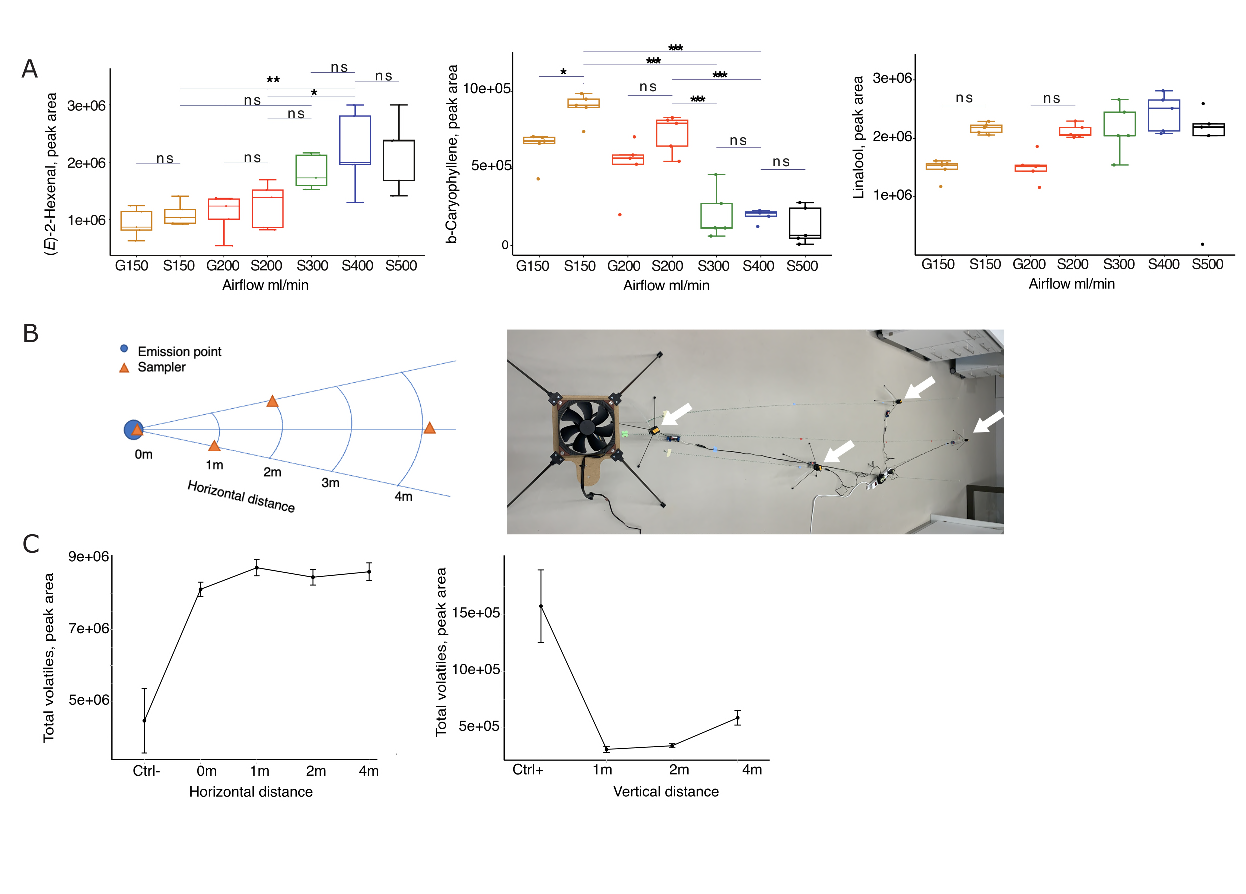
\includegraphics[width=0.99\textwidth]{figures/OUTDOOR_PAPER_FIGURE_pumps_v01.eps}
\includegraphics[width=0.99\textwidth]{chapters/papers/VOL/figures/fig-4-results/figure_4_pumps.eps}
% \vspace{-6em}
\caption{Results of volatile sampling and testing. (A) Comparisons between our sampler (S) and a commercial pump (G, GilAir plus), and patterns of volatile recovery at increasing airflow rates. Results of Bonferroni-corrected pairwise contrasts after multivariate analysis of variance (df = 6, 28; Pillai = 2.64; \textit{F} = 3.04; \textit{P} = 0.0001) are shown within each boxplot; ns indicates non-significant differences. Statistical differences are denoted as \textit{P} = 0.01 *, \textit{P} = 0.001 **, and \textit{P} = 0.0001 ***. (B) Schematic and photo of the horizontal distance sampling performed in the laboratory. The fan observed in the photo was used to imitate the air downwash of a drone hovering on top of the source for the vertical distance testing. The patterns observed in the plots correspond to the sum of volatiles collected at different horizontal and vertical distances from the source plus negative (no volatiles) and positive (volatiles without air downwash) controls, respectively. The plots show the mean and standard error.}
\label{Flowrate_results}
\end{figure*}



Overall, we found that the GilAir plus pump and our six times lighter sampler performed comparably at the airflows of 150 and 200~ml/min (Figure S1 and Figure \ref{Flowrate_results}A). The observed differences between the two pumps at 150~ml/min in the volatile compounds $\beta$-caryophyllene (Figure \ref{Flowrate_results}A), TMTT and eugenol (Figure S1) indicate that our sampler collected higher quantities of these compounds. This finding may be related to these three compounds having the lowest volatility, as they have the highest boiling points among the tested volatiles: $>$~200~°C, while the rest have boiling points of $<$~200~°C under atmospheric pressure (760~mm~Hg). 
Furthermore, we found that airflow rates above 200~ml/min affected the concentration of the volatiles differently, with similar patterns for compounds having more similar structures. Such patterns suggest that with higher flow rates, it is possible to either collect 1) increasing quantities, as for (\textit{E})-2-hexenal, 2) decreasing quantities, as for $\beta$-caryophyllene, or 3) collect the same quantities regardless of the airflow rate used, as for linalool (Figure \ref{Flowrate_results}A). The intrinsic properties of the volatile compounds may explain these patterns. For instance, considering the two benzenoids tested: eugenol has a boiling point (bp) of 254~°C at atmospheric pressure and behaves similarly to the sesquiterpene $\beta$-caryophyllene (bp: 245~°C) and TMTT (bp: 293~°C), while p-cymene has a bp of 177~°C, and behaves similar to the GLVs (\textit{E})-2-hexenal (bp: 146~°C) and (\textit{Z})-3-hexenyl acetate (76~°C) (Figure S1). Moreover, the lack of differences in volatile quantity at the highest airflow rates of 300, 400 and 500 ml/min suggest no advantages of increasing flow rates above 300 ml. The patterns indicate that the best compromise would be sampling at 200-300~ml/min. This sampling rate would increase the likelihood of collecting higher concentrations of the GLVs and the benzenoids, at the cost of recovering lower concentrations of the sesquiterpene and the norditerpene (Figure S1). These results are valuable in demonstrating that different airflows might have differential impacts on the plant volatiles of interest. However, the question of what airflow represents the best compromise for the researcher will ultimately depend on biological relevance of the volatile compounds to be sampled. For instance, in our tests, we included 5 volatile compounds (exceptions are p-cymene and eugenol, included for structural variety) that are consistent and frequently found to be emitted upon insect herbivore damage to maize plants. The GLVs are the first plant volatiles emitted by maize seedlings upon herbivore damage, commonly released within the first 90~min and peaking at 45~min, while mono- and sequiterpenoids are emitted much later, peaking around 500 min after damage \cite{erb_indole_2015}. This suggests that sampling at an airflow rate of 300~ml/min in a maize field could help us detect early signals of herbivore damage when focusing on the GLVs, but a lower airflow might be better when focusing on larger and more slowly released terpenoids, which can be more specific indicators, as many GLVs are commonly released by damaged plants. 

\subsection{Effect of Horizontal Distance on Volatile Sampling}

To better understand the effect of the horizontal distance from the sampler to the volatile emission point on the qualitative and quantitative recovery of the volatile compounds, we collected headspace samples at distances of 1~m, 2~m, and 4~m from the volatile source at ground level. These tests were performed under indoor conditions of still air at a mean temperature of 21.6°C and relative humidity of 24\%. The airflow of the sampler was set to 300~ml/min with a Tenax-TA\textsuperscript{TM} filter attached, and a total air volume of 5~l was collected over 16.66 minutes. Five replicates per distance as well as controls were taken. In each replicate, 0.5~$\upmu$l of the volatile blend containing the above-mentioned seven volatile compounds was added to a Whatman\textsuperscript{TM} filter paper at the moment of starting the sampler at the corresponding distances. For the horizontal distance testing, we included a negative control in which no volatiles were added to the filter paper. The negative controls were intended to sample room air and to control for possible contamination during sampling, i.e., to account for the influence of volatiles that were not part of our blend of standard volatiles (Figure \ref{Flowrate_results}C, horizontal distance barplot). These negative control samples were taken at the 0~m point, and were taken at the beginning and at the end of the sampling day, and in between every 3-4 volatile samplings to cover the whole sampling period.
Overall, no statistical differences were found in the concentration of any of the volatiles at different horizontal  distances to the sampler (see Figure S2 for patterns per volatile compound). This finding is well summarized in the sum of all volatiles tested, therefore in Figure \ref{Flowrate_results}B, we present and discuss patterns in the total volatiles recovered per control and distance. For the horizontal distance testing, the data suggest that total volatile quantity is not affected even at 4~m distance from the volatile emission point. However, it is interesting to note that less volatiles were collected at the closest distance tested (0 m) compared to 1, 2, and 4 m. This may be explained by the compounds' diffusion in air \cite{Schuman2023}. These findings can help in the development of scalable volatile-based remote sensing by informing about the effects of horizontal (ground) distance from the sampler to the potential source of volatile emission (i.e., plants) on the detection and concentration of the volatiles depending on their chemical properties.



\subsection{Effect of Downwash on Volatile Sampling}
%
We examined the effect that the downwash of a UAV hovering at different heights above the volatile sampler could have on the volatiles. The volatile collection was done in the laboratory to maintain the same air temperature and still air conditions as in the horizontal distance testing. For this reason, we first recorded the air velocity induced by the downwash of a DJI Mavic Pro drone hovering over the sampler with an anemometer (Testo 405i) at 1, 2 and 4 m. These recordings were done indoors and under still air conditions. This allowed us to then calibrate a Noctua NF-A14 PPC 3000 PWM fan to produce air velocities equivalent to the downwash at the three above-mentioned vertical distances (see Supplementary Material for more details). For the vertical distance test, we had positive and negative control samples. The negative controls were intended to sample room air and to control for possible contamination during sampling, i.e., to account for the influence of volatiles that were not part of our blend of standard volatiles (results not shown in Figure \ref{Flowrate_results}C, vertical distance barplot,  but see Table S1 for statistics). The positive controls consisted of volatile sampling without downwash and with the filter paper impregnated with the blend of standard volatiles. The positive control was used as a baseline to compare the effects of downwash to that of still air and thus to know the quantity of volatiles being collected under the same room and setup conditions. Control samples were taken at the beginning and at the end of the sampling day, and in between every 3-4 volatile samplings to cover the whole sampling period. During sampling, the same procedure described above for the horizontal testing was followed (see also the Supplementary Material). The average air velocities were 1.34~m/s at 1~m vertical distance, 1.08~m/s at 2~m, and 0.56~m/s at 4~m. At all three simulated vertical distances, most of the volatile compounds were recovered at significantly lower quantities compared to the positive control (Table S1, Figure S2 and \ref{Flowrate_results}B). This demonstrates that the downwash of a hovering UAV during sampling can limit the qualitative and quantitative analysis of the volatile compounds, thus supporting the development of the method based on placing and re-collecting the sampler.



\subsection{Outdoor Robotic Deployment Accuracy and Retrieval Repeatability}
\label{robotic_deployment_and_retrieval}

% \subsubsection{Outdoor Deployment Accuracy and Retrieval Repeatability Tests}

\begin{table}[!ht]
% increase table row spacing, adjust to taste
\renewcommand{\arraystretch}{1.0}
% if using array.sty, it might be a good idea to tweak the value of
% \extrarowheight as needed to properly center the text within the cells
\caption{Deployment Accuracy}
\label{table-4-deployment-accuracy}
\centering
% Some packages, such as MDW tools, offer better commands for making tables
% than the plain LaTeX2e tabular which is used here.
\begin{tabular}{ccc}
$\overline{x}$ (cm) & $\overline{y}$ (cm) & $\overline{WS}_D$ (m/s) \\
\hline
1.4 \textpm 6.04 & 2.9 \textpm 5.59 & 1.71\\
\end{tabular}
\end{table}

\begin{table}[!ht]
% increase table row spacing, adjust to taste
\renewcommand{\arraystretch}{1.0}
% if using array.sty, it might be a good idea to tweak the value of
% \extrarowheight as needed to properly center the text within the cells
\caption{Retrieval Repeatability}
\label{table-5-retrieval-repeatability}
\centering
% Some packages, such as MDW tools, offer better commands for making tables
% than the plain LaTeX2e tabular which is used here.
\begin{tabular}{ccc}
Retrieval (\%) & $\overline{WS}_R$ (m/s) & Retrieval Time (s)\\
\hline
91.6 & 0.35 \textpm 0.26 & 61.67 \textpm 16.91\\
\end{tabular}
\end{table}

The deployment accuracy of the sampler was tested using an A0 grid ($n=10$) with a central red target (Figure~\ref{fig-5-deployment-accuracy}A), and the deviation to the center measured to the nearest centimeter (Figure~\ref{fig-5-deployment-accuracy}B). The UAV, a DJI Mavic Pro, was piloted manually, with the assistance of the onboard downward-facing camera (Figure~\ref{fig-5-deployment-accuracy}C-E). The UAV started 5~m (horizontal) from a ground target, ascended to an altitude of 10~m, then descended towards the target and was centered on it with the camera feedback to deploy the sampler. The results are shown in Figure~\ref{fig-5-deployment-accuracy}B. Table~\ref{table-4-deployment-accuracy} shows the mean and standard deviation from the center in the x and y directions ($\overline{x}$, and $\overline{y}$) and the mean wind speed during deployments ($\overline{WS}_D$). These results show that, even with manual piloting, the sampler can be placed consistently within 10~cm of the target. A video of the deployment process is available as supplementary material.

\begin{figure}[!hpt]
\centering
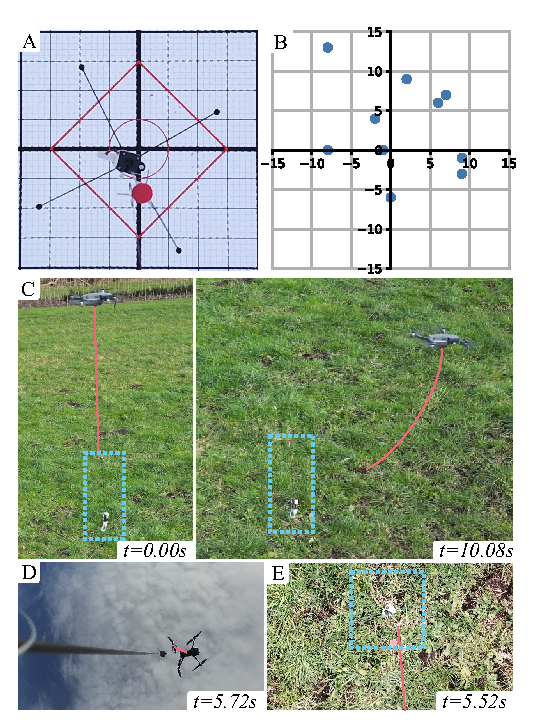
\includegraphics[width=0.9\columnwidth]{chapters/papers/VOL/figures/fig-5-deployment-accuracy/fig-5-deployment-accuracy.eps}
\caption{Deployment accuracy and outdoor test. (A) Deployment: downward-facing UAV camera view of the sampler descending on the target, the red dot is the top of the sampler hook assembly. (B) Scatter plot of sampler locations after being deployed with the UAV ($n=10$), in cm. (C) Deployment process: (left) sampler suspended beneath the UAV, (right) sampler successfully deployed (red wire highlighted for clarity). (D) Upward-facing sampler view after deployment. (E) Downward UAV view after deployment.}
\label{fig-5-deployment-accuracy}
\end{figure}

\begin{figure}[!hpt]
\centering
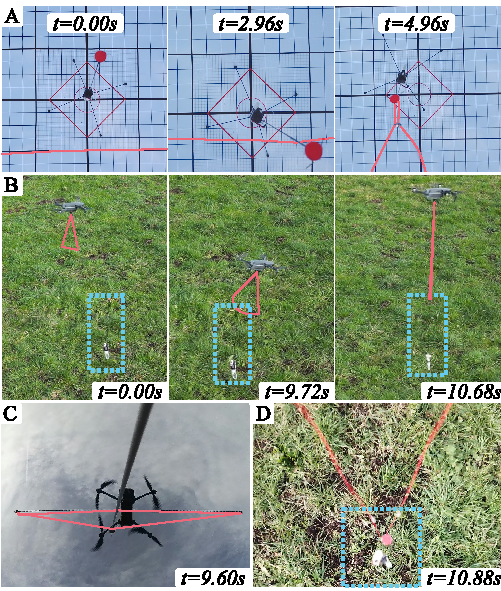
\includegraphics[width=0.9\columnwidth]{chapters/papers/VOL/figures/fig-6-retrieval-success/fig-6-retrieval-success.eps}
\caption{Retrieval success and outdoor test. (A) Retrieval: downward camera feed during sampler collection, from left to right: approaching sampler, string ready to engage, and sampler collected (red wire highlighted for clarity). (B) Outdoor retrieval with approach, wire engaging on the hook, and successful retrieval (from left to right). (C) Upward-facing sampler view when the wire engages. (D) Downward UAV view after successful retrieval.}
\label{fig-6-retrieval-success}
\end{figure}

To test the repeatability of retrieval, the sampler was placed on the target and then retrieved with the UAV, also piloted manually. The percentage of successes  ($11/12$) is shown in Table~\ref{table-5-retrieval-repeatability}, along with mean wind speed during retrievals ($\overline{WS}_R)$. Similar to the deployment, the UAV takes off, flies to 10~m altitude, flies to the sampler, descends and collects it, then returns to the take-off location to deposit the sampler (see Figure~\ref{fig-6-retrieval-success}). A retrieval is considered a success if the sampler is collected from the target and placed on the designated area next to the take-off pad with the retrieval mechanism properly engaged. There were three practice runs before the experiment. The single failure case during the experiment occurred when the sampler was laterally misaligned, such that it hooked onto one of the magnets, which caused the other magnet not to disengage. This was counted as a failure, even though the sampler remained attached and returned to the take-off pad. A video of the retrieval process is available as supplementary material.
%The mean temperature during the retrieval experiments was measured as 5.98 \textpm 2.89, although the sun was shining on the sensor, and weather forcasts place the temperature closer to -2 C

% \begin{table}[!t]
% % increase table row spacing, adjust to taste
% \renewcommand{\arraystretch}{1.0}
% % if using array.sty, it might be a good idea to tweak the value of
% % \extrarowheight as needed to properly center the text within the cells
% \caption{Deployment Accuracy and Retrieval Repeatability}
% \label{table-4-accuracy-and-repeatability}
% \centering
% % Some packages, such as MDW tools, offer better commands for making tables
% % than the plain LaTeX2e tabular which is used here.
% \begin{tabular}{ccccc}
% $\overline{x}$ (cm) & $\overline{y}$ (cm) & $\overline{WS}_D$ (m/s) & Retrieval (\%) & $\overline{WS}_R$ (m/s)\\
% \hline
% 1.4 \textpm 6.04 & 2.9 \textpm 5.59 & 1.71 \textpm 3.12 & 91.6 & 0.35 \textpm 0.26 \\
% \end{tabular}
% \end{table}



\subsection{Outdoor Volatile Collection from Damaged Maize Plants}
\label{outdoor_volatile_collection}

\begin{figure*}[!pht]
\centering
% \includegraphics[width=1\columnwidth]{figures/OUTDOOR_PAPER_FIGURE_outdoors.eps}
% 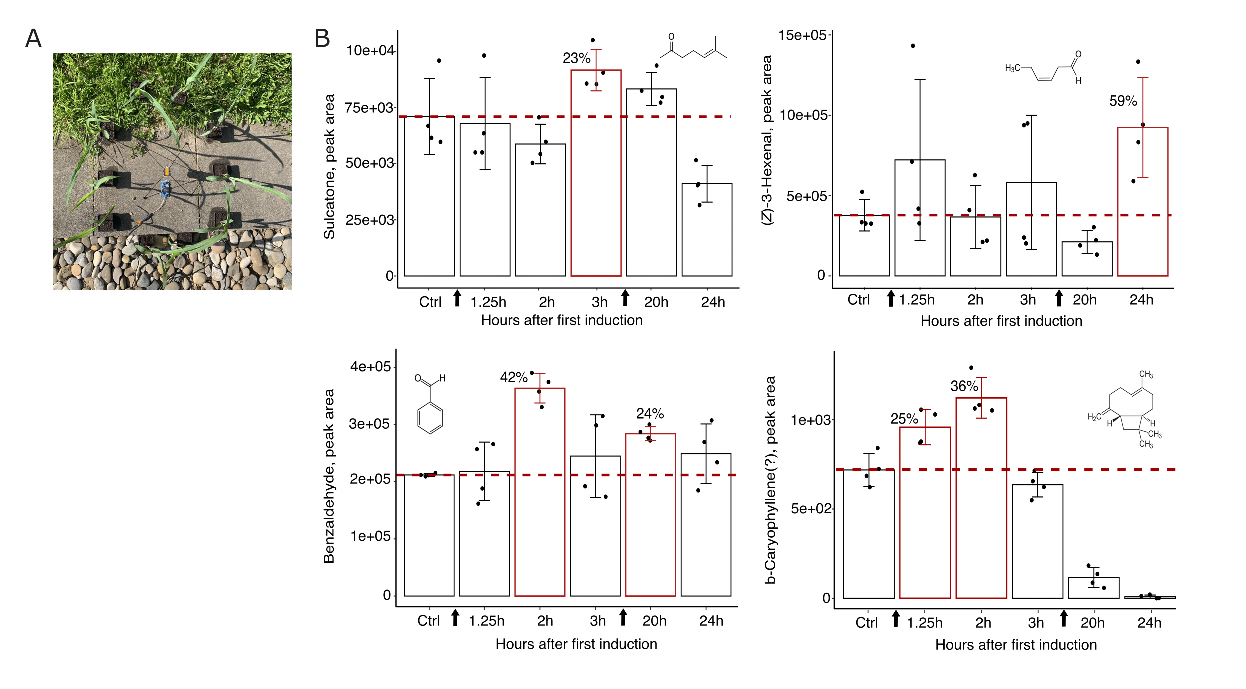
\includegraphics[width=0.99\textwidth]{figures/OUTDOOR_PAPER_FIGURE_outdoors_v01.eps}
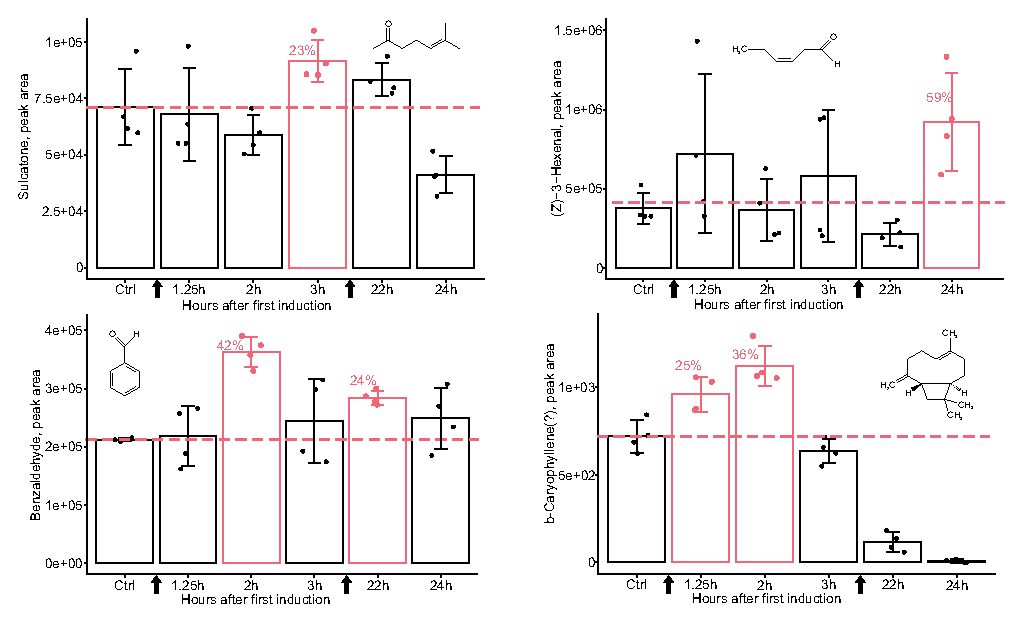
\includegraphics[width=0.99\textwidth]{chapters/papers/VOL/figures/fig-4-results/figure_4_outdoor.eps}
% \vspace{-6em}
\caption{Outdoor volatile collection from maize plants with simulated insect herbivore damage. The barplots show the four volatile compounds from which a significant increase upon induction was found. The dotted line crossing the bars horizontally indicates the mean of the control samples, and is intended to aid in visualizing the significant increases upon induction at different times (indicated in red and percentages). The individual dots represent each of the replicates (i.e., a sampler with its 10 plants). The arrows in the x-axis pointing upwards indicate the two simulated herbivory events (i.e., at 10:00 a.m. on the first days, and at 07:00 a.m. on the next day after the first induction). For full statistical results refer to Table S2 and Figure S5. The identification of $\beta$-caryophyllene is tentative and based on comparison to mass spectra generated from analytical standard compounds.}
\label{fig:outdoor_testing}
\end{figure*}

We tested whether our samplers were capable of recovering volatiles emitted from maize plants exposed to simulated insect herbivory damage outdoors. For this experiment, 15-day-old maize plants (\textit{Zea mays} var. Delprim) placed outdoors were damaged, and volatiles collected with our light-weight samplers at different time periods. The maize plants were grown in individual pots at 24°C and 50\% relative humidity in the greenhouse facilities at University of Zurich Irchel campus. To induce the plants, we imitated insect herbivore damage with mechanical damage and application of insect regurgitant to wounds \cite{Waterman2019}. The mechanical damage on the leaves was performed by scratching the leaves with fine sandpaper (100 grit) and fine tweezers (Figure S3). The regurgitant of the Egyptian cotton leafworm \textit{Spodoptera littoralis} from L4 and L5 larvae stages was used (10~$\upmu$l per plant; see Supplementary Materials \cite{Geckeler2023} for details).
The experiment consisted of placing 10 plants in a circle around each of the four samplers at a distance of ca. 30~cm from the sampler (Figure S3). This occurred at 08:30 a.m., and the plants and samplers were placed in a green area outside the greenhouse (Figure S3). We conducted a total of six sampling intervals of 30 min., replicated 4 times each using the lightweight samplers at an airflow of 300~ml/min. The first sampling was done at time -1 (09:00 a.m.) when the plants were not yet induced with simulated herbivory. We considered this sampling as the control, and the volatiles recovered would be interpreted as volatiles emitted mostly from the surrounding maize plants, but caution is needed with this interpretation as other surrounding plants could have also contributed to the collected volatiles. The control samples are thus expected to represent constitutively emitted plant volatiles, emitted in the absence of stress, as well as background volatiles from surrounding vegetation. We consider this as the basal level from which an increase in volatile emissions – as a result of damage – can be compared. Volatiles that significantly increase their emission compared to constitutive levels are thus called induced volatiles. During the experiment, the plants were induced twice with simulated insect herbivory damage and regurgitant. The first stress induction was done at 10:00 a.m., and the second stress induction was done at 07:00 a.m. the next day (Figure \ref{fig:outdoor_testing}).
Overall, we could identify eight volatile compounds from our outdoor samples (Figure S4, Table S2). From these volatiles, we detected a significant increase upon simulated herbivory in four of them (Figure \ref{fig:outdoor_testing}). Interestingly, the timing at which these compounds reached their highest abundance in our samples differed greatly. For instance, three compounds showed a significant increase upon the first induction compared to the control. Sulcatone (a ketone) showed an increase after 3 h, while $\beta$-caryophyllene (sesquiterpene) and benzaldehyde (benzenoid) increased within 2 h of the first induction (Figure \ref{fig:outdoor_testing}). On the other hand, we found that only two compounds significantly increased the day after the first induction and upon a second round of simulated herbivory. Benzaldehyde again showed an increase, but much less than its increase after the first induction, while the GLV (\textit{Z})-3-hexenal showed a dramatic increase only after the two rounds of induction. Although our results are preliminary, the findings suggest that these four volatile compounds could represent promising indicators for early warning of insect pest presence in maize fields. They also demonstrate the sampler's suitability for collecting plant volatiles under outdoor conditions. 

\section{Discussion}
Plant volatiles present a promising alternative to conventional remote sensing techniques for the early detection of plant stress. In this work we demonstrated the successful collection of plant volatiles with our sampler, both under stable laboratory temperature and air conditions as well as under variable outdoor conditions. We also showed the successful deployment and retrieval of the sampler with a UAV. To ensure repeatability for characterization of the sampler, known mixes of volatile standards were prepared and utilized during the tests and also used to indicate sensitivity to UAV downwash and distance from source. We also provided preliminary results on the sensitivity of detection and identity potential volatile indicators for herbivore presence and damage diagnosis under realistic conditions. Considering the active sampling volume of 5~l, the passive exposure of the filter to ambient air during transit is considered negligible \cite{mckinney_sampler_2019}, and this will be confirmed in future control flights. For studies requiring more precise measurements, gas-tight isolation of the sampling tube under an appropriate protective atmosphere during transit should be considered.
Since retrieval and collection are two separate mechanisms, future work will look at combining them in a single passive mechanism or introducing an additional actuator to avoid having to switch between them.
The sampler uses a hook extending above the pump assembly for retrieval and deployment. This extension and the sampler legs are dimensioned for the target crop, young maize. To broaden the application for different crops and growth stages, alternate mechanisms for retrieval and collection are under investigation. 
Current piloting of the UAV was done manually; autonomous flight, deployment, and retrieval procedures with the current deployment and collection mechanisms are the subject of ongoing work. Despite manual piloting, the sampler could be placed with 10~cm accuracy. Increased accuracy, robustness, and repeatability of sampler retrieval can be expected by utilizing increased autonomy, for instance, autonomous UAV alignment using GPS with visual servoing for fine-tuning.

\section{Conclusion}
Here, we present a novel lightweight and UAV-deployable sampler for the spatial collection of plant volatiles suitable for field conditions. This approach makes sampling independent of ground accessibility and minimizes disturbance to plants; thus, it is suitable for more complex field designs with little bare ground as in sustainable intensification and could be of interest for other remote sampling applications. The current prototype is lightweight, under 100~g, and can be deployed with a UAV under manual operation with 10~cm accuracy. The sampler can also be re-collected with the UAV, paving the way for fully autonomous sampler deployment and collection in agricultural fields at scale. Furthermore, we demonstrate that the performance of our low-cost sampler is comparable to that of a commercial portable pump in terms of the qualitative and quantitative collection of volatile compounds of diverse chemical classes. Indeed, our sampler outperformed the commercial pump at higher air flow rates, which could be an advantage when sampling outdoors under conditions of expected air disturbance. 
Horizontal distance up to four meters did not seem to have an effect on collected volatiles, which might in part be explained by how volatiles diffuse through air. 
UAV downwash from any height negatively impacted all volatile collection qualitatively and quantitatively, demonstrating the need for the deployable sampler. Finally, we were able to demonstrate that our sampler is capable of recovering volatiles from maize plants with simulated herbivory even under constantly changing conditions outdoors (i.e., wind, light, humidity). Our results are promising in suggesting that at least four volatile compounds emitted by stressed plants during the first hours can potentially be indicators of early insect pest activity.

With the described UAV-based volatile sampling, we hope to contribute to the practical use of plant volatiles in agriculture as early indicators of plant stress. In combination with other remote sensing techniques, this will allow optimized interventions by reducing pesticide use and costs to the farmer, and increase yield under sustainable intensification strategies towards more efficient crop production. 

\section*{Acknowledgments}
This work was supported by Syngenta through the Plant Science Center-Syngenta Fellowship Program (grant to M. C. Schuman and S. Mintchev), and from the SNSF Eccellenza Grant N.186865 (grant to S. Mintchev). We would like to thank Anke Buchholz for insightful feedback and discussions. We appreciate the guidance of Jakob Lang and Matteo Krummenacher for the  development of the method used for TD-GC-MS analyses. We would also like to thank Luca Girardi for drone videography equipment.

 
% argument is your BibTeX string definitions and bibliography database(s)
% \bibliographystyle{IEEEtran}
% \bibliography{bibtex/nourl,bibtex/Plant-Eco-Air,bibtex/references-mendeley,bibtex/Merry}
%

